\section{Estudio teórico}

\subsection{Técnicas utilizadas}

\begin{frame}{Estudio teórico}{Técnicas utilizadas - Segmentación de objetos en primer plano}

\begin{itemize}
    \justifying
    \item Obtener una imagen que se encuentre en el fondo sin ningún objeto en movimiento.
    \item El modelo de representación debe ser robusto ante posibles alteraciones en la iluminación u objetos que han sido introducidos y/o retirados.
    \item Dos principales problemas: detección de cambios y la detección de movimientos.
\end{itemize}


\begin{figure}[ht]
\centering
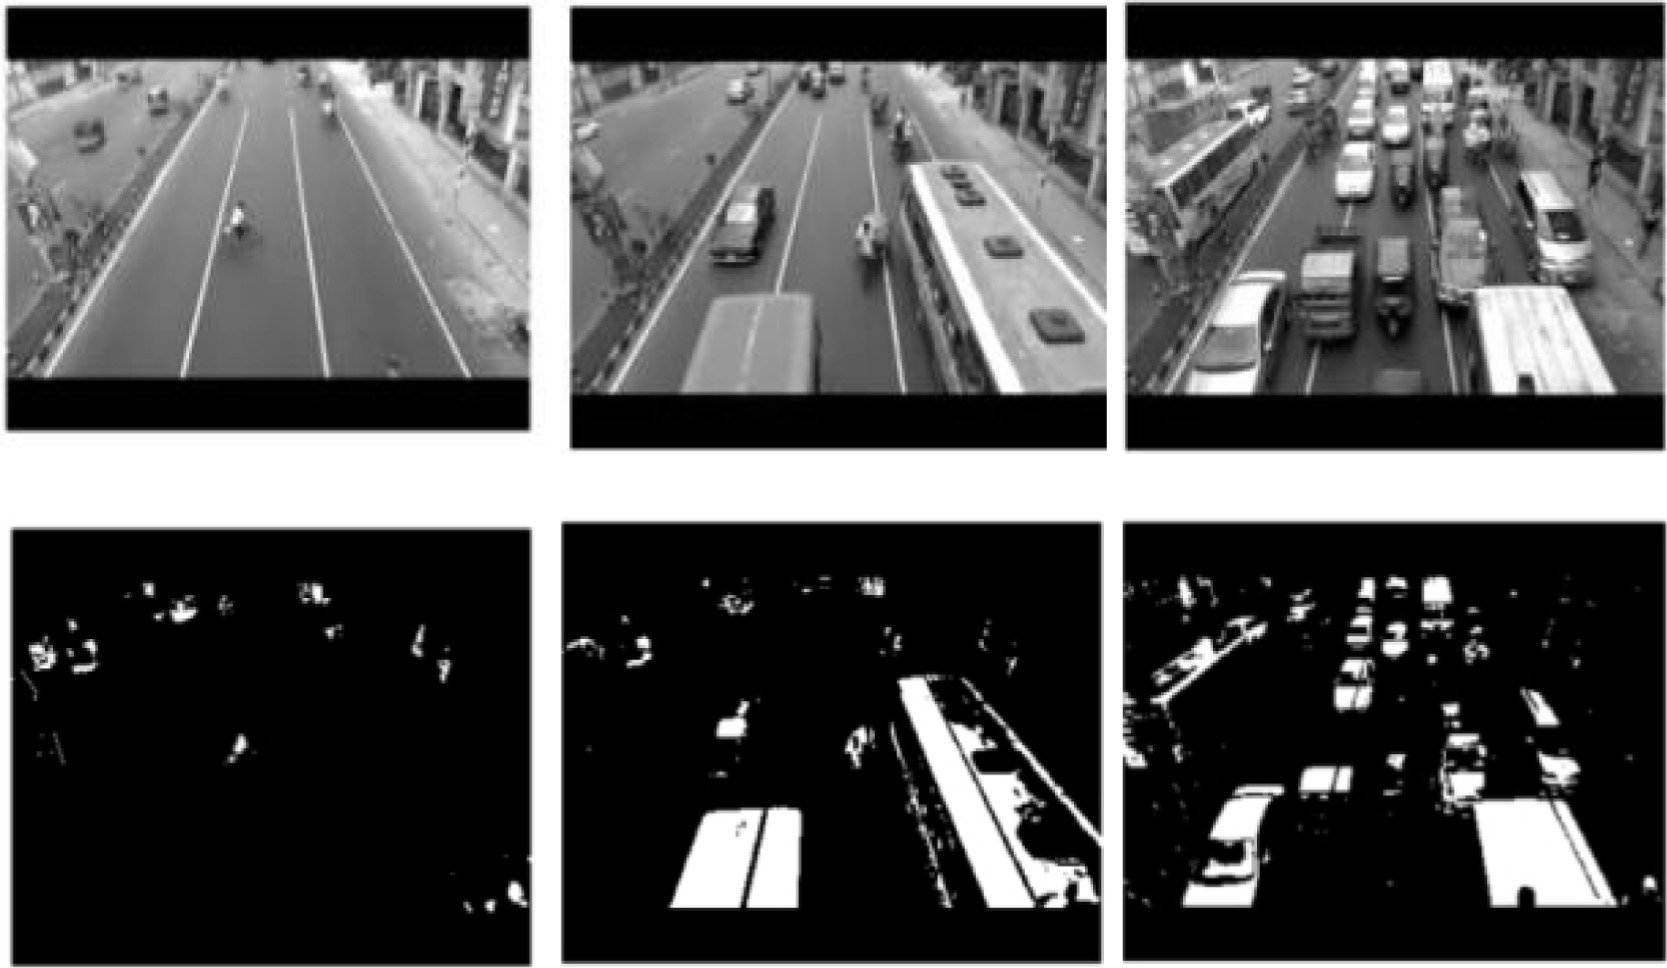
\includegraphics[width=0.4\textwidth]{Images/estudio-teorico/background-subtraction-example.jpg}
\caption{\label{fig:background-subtraction-example}Ejemplo sustracción del fondo}
\end{figure}

\end{frame}

%%%%%%%%%%%%%%%%%%%%%%%%%%%%%%%%%%%%%%%%%%%%%%%%%%%%%%%%%%%%%%%%%

\begin{frame}{Estudio teórico}{Técnicas utilizadas - Detección de objetos estacionarios}

\begin{figure}[ht]
\centering
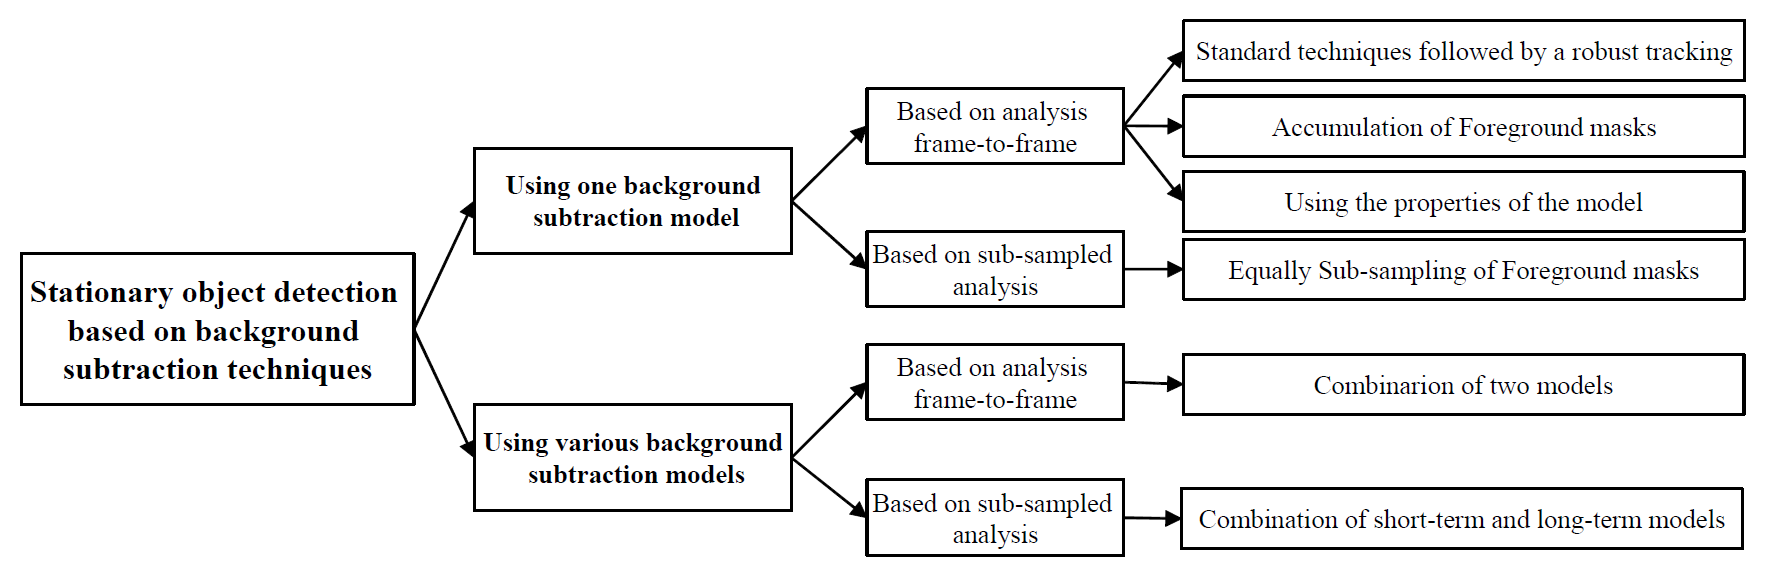
\includegraphics[width=1\textwidth]{Images/estudio-teorico/metodos-sustraccion-fondo-deteccion-fondo-estacionario.png}
\caption{\label{fig:metodos-sustraccion-fondo-deteccion-fondo-estacionario}Clasificación de sustracción del fondo basados en métodos de detección de objetos estacionarios}
\end{figure}

\end{frame}

%%%%%%%%%%%%%%%%%%%%%%%%%%%%%%%%%%%%%%%%%%%%%%%%%%%%%%%%%%%%%%%%%

\begin{frame}{Estudio teórico}{Técnicas utilizadas - Reconocimiento del comportamiento}

\begin{itemize}
    \justifying
    \item La detección de comportamientos anormales en la videovigilancia es un reto en la visión por computadora y últimamente ha experimentado importantes avances.
    \item Las etapas de procesamiento no permiten comprender el tipo de acción que realiza el objeto en movimiento ni determinan si su
comportamiento es normal o no.
    \item Densidad de escenas e interacción de objetos en movimiento.
    \item Métodos de clasificación: supervisado, semi-supervisado y no supervisado.
\end{itemize}

\begin{columns}

  \begin{column}{0.5\textwidth}
    \begin{figure}[ht]
    \centering
    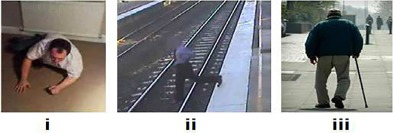
\includegraphics[width=0.65\textwidth]{Images/estudio-teorico/Abnormal-behaviors-single-person.jpg}
    \caption{\label{fig:Abnormal-behaviors-single-person}Comportamientos anómalos en una persona}
    \end{figure}
  \end{column}
  
  \begin{column}{0.5\textwidth}  %%<--- here
    \begin{figure}[ht]
    \centering
    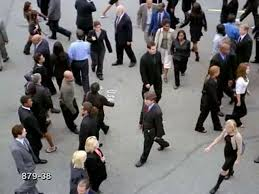
\includegraphics[width=0.5\textwidth]{Images/estudio-teorico/abnormal-behaviors-crowded-scene.jpg}
    \caption{\label{abnormal-behaviors-crowded-scene}Comportamientos anómalos en múltiples personas}
    \end{figure}    
  \end{column}
  
\end{columns}

\end{frame}

%%%%%%%%%%%%%%%%%%%%%%%%%%%%%%%%%%%%%%%%%%%%%%%%%%%%%%%%%%%%%%%%%

\begin{frame}{Estudio teórico}{Técnicas utilizadas - Detección de personas y objetos}

\begin{itemize}
    \justifying
    \item Los algoritmos de detección de personas y objetos se clasifican según el enfoque utilizado para generar o extraer los objetos iniciales y en base al modelo de persona.
    \item La segmentación genera directamente los objetos candidatos a ser persona u objetos y fácilmente se rechaza las áreas irrelevantes de la imagen, es decir, sin objetos de interés.
    \item La búsqueda exhaustiva consiste en escanear la imagen completa buscando similitudes con el modelo de persona elegido en múltiples escalas y ubicaciones.
\end{itemize}

\begin{figure}[ht]
\centering
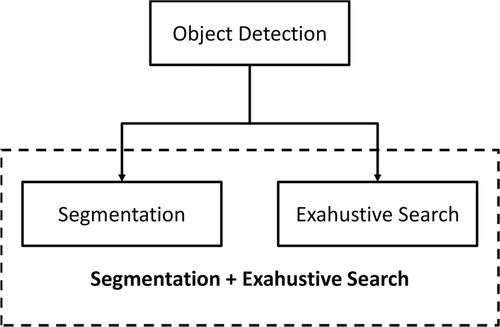
\includegraphics[width=0.4\textwidth]{Images/estudio-teorico/people-detection-classification.png}
\caption{\label{fig:people-detection-classification}Clasificación en la detección de personas}
\end{figure}

\end{frame}

%%%%%%%%%%%%%%%%%%%%%%%%%%%%%%%%%%%%%%%%%%%%%%%%%%%%%%%%%%%%%%%%%

\subsection{Algoritmos de detección y seguimiento elegidos}

\begin{frame}{Estudio teórico}{Algoritmo de detección de objetos YOLOv4}

\justifying
En vista a las métricas se puede concluir que, de todos los detectores de objetos en tiempo real actuales, YOLOv4 es el mejor en términos de velocidad y precisión.

\begin{figure}[ht]
\centering
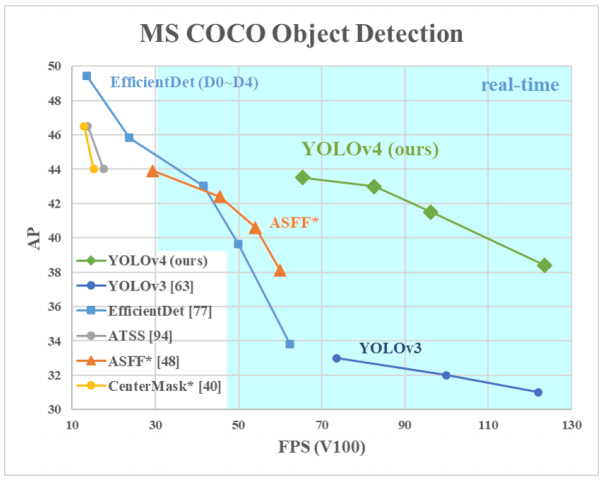
\includegraphics[width=0.5\textwidth]{Images/estudio-teorico/yolov4-vs-others.png}
\caption{\label{fig:yolov4-vs-others}YOLOv4 frente a otros detectores}
\end{figure}

\end{frame}

%%%%%%%%%%%%%%%%%%%%%%%%%%%%%%%%%%%%%%%%%%%%%%%%%%%%%%%%%%%%%%%%%

\begin{frame}{Estudio teórico}{Algoritmo de detección de objetos YOLOv4}

\begin{itemize}
    \justifying
    \item La detección primero divide la imagen en una cuadrícula de SxS.
    \item En cada una de las celdas se predice N posibles cuadros delimitadores y se calcula el nivel de certidumbre.
    \item Se eliminan las cajas que estén por debajo de un límite.
    \item A los cuadros restantes se les aplica un paso de ``non-max suppression''.
\end{itemize}

\begin{figure}[ht]
\centering
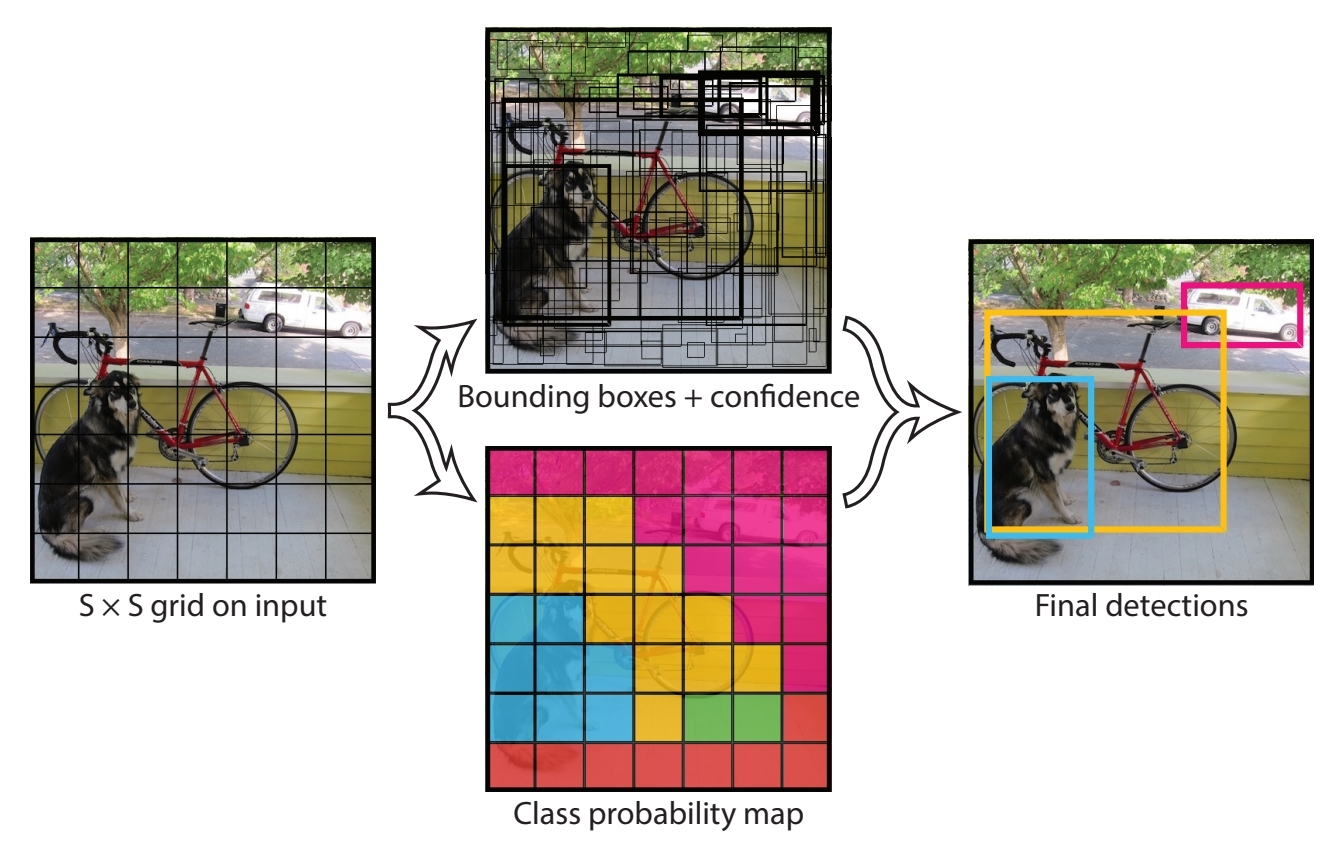
\includegraphics[width=0.49\textwidth]{Images/estudio-teorico/funcionamiento-yolo.jpg}
\caption{\label{fig:funcionamiento-yolo}Funcionamiento del algoritmo YOLO}
\end{figure}

\end{frame}

%%%%%%%%%%%%%%%%%%%%%%%%%%%%%%%%%%%%%%%%%%%%%%%%%%%%%%%%%%%%%%%%%

\begin{frame}{Estudio teórico}{Algoritmo de seguimiento de objetos Deep SORT}

\begin{itemize}
    \justifying
    \item Utiliza los pesos pre-entrenados de YOLOv4 para extraer los cuadros delimitadores de las detecciones.
    \item Los cuadros delimitadores sirven de entrada al algoritmo SORT para realizar el seguimiento. % Algoritmo SORT basado en el Filtro de Kalman
    \item Mediante una \textbf{DNN} entrenada el algoritmo asocia los \textit{tracks} activos y los que se han perdido.
\end{itemize}

\begin{figure}[ht]
\centering
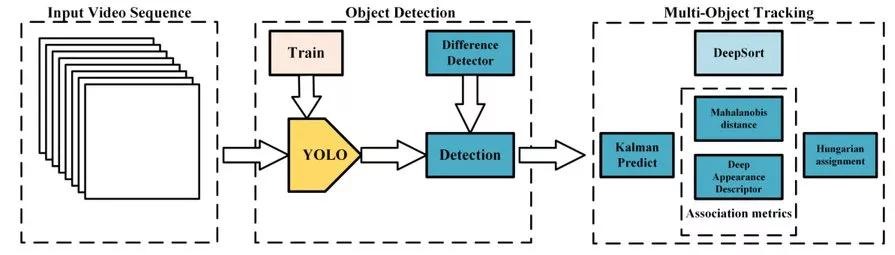
\includegraphics[width=0.75\textwidth]{Images/estudio-teorico/yolo-deepsort-scheme.jpg}
\caption{\label{fig:yolo-deepsort-scheme}Esquema etapas detección y seguimiento con YOLOv4 y Deep SORT}
\end{figure}

\end{frame}
